\documentclass[tikz,border=4pt]{standalone}
\usepackage{tikz}
\usetikzlibrary{arrows.meta,calc,positioning}

\definecolor{perceptionfill}{RGB}{238,248,246}
\definecolor{perceptionline}{RGB}{31,122,114}
\definecolor{estimatorfill}{RGB}{239,244,252}
\definecolor{estimatorline}{RGB}{50,91,143}
\definecolor{controllerfill}{RGB}{253,245,235}
\definecolor{controllerline}{RGB}{176,102,32}

\begin{document}
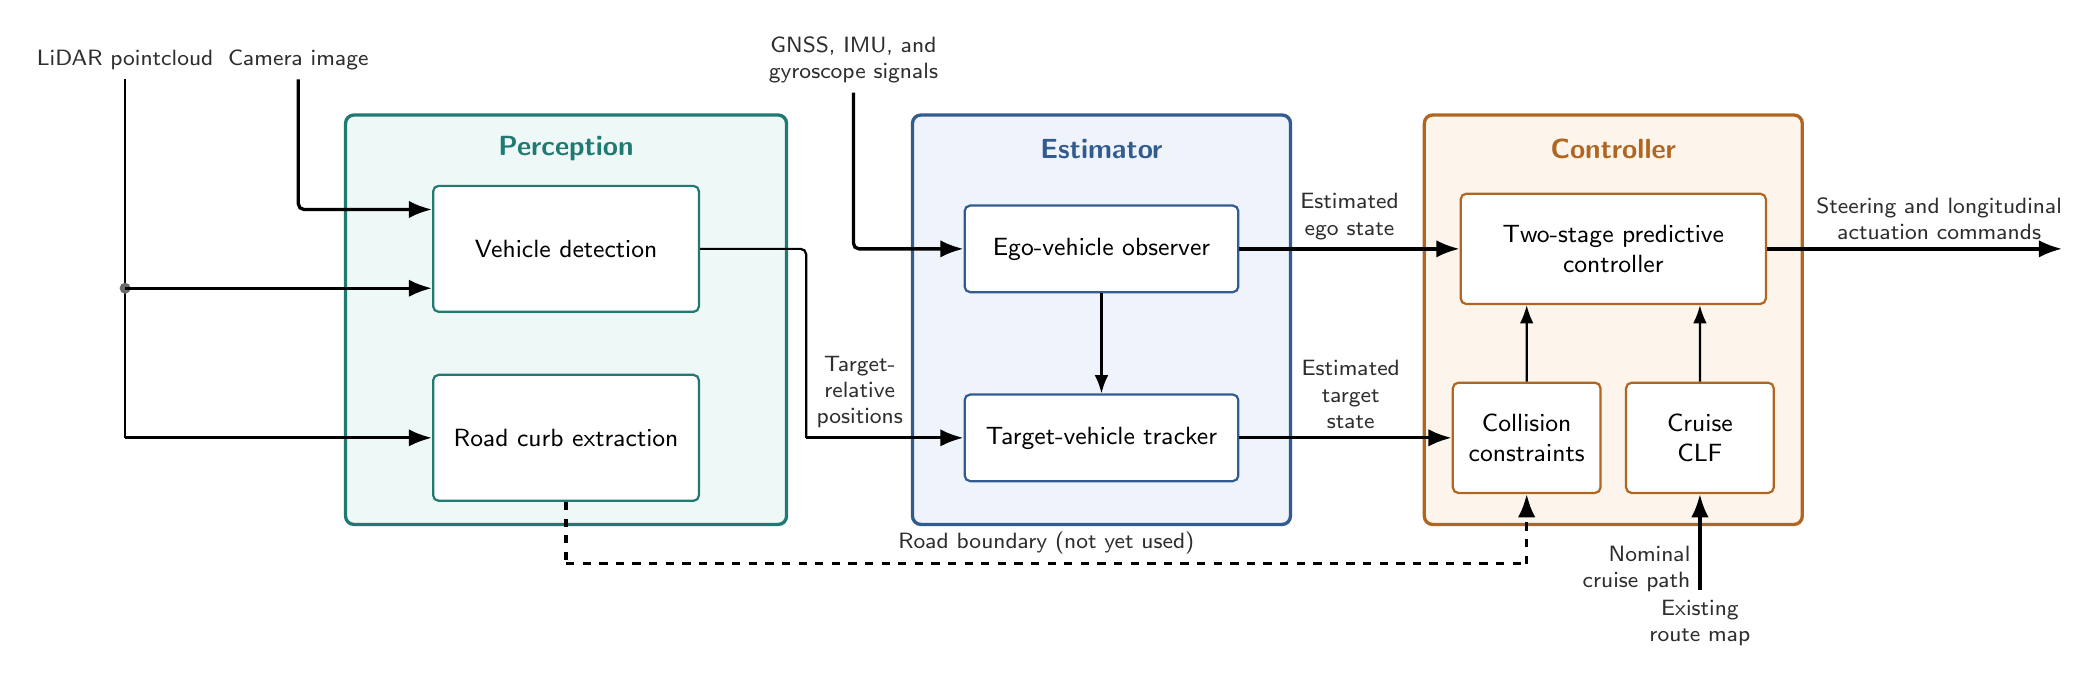
\begin{tikzpicture}[
    font=\sffamily\small,
    >=Latex,
    component/.style={
        rounded corners=3pt,
        very thick,
        minimum width=48mm,
        minimum height=52mm
    },
    perceptionComponent/.style={
        component,
        minimum width=56mm,
        draw=perceptionline,
        fill=perceptionfill
    },
    estimatorComponent/.style={
        component,
        draw=estimatorline,
        fill=estimatorfill
    },
    controllerComponent/.style={
        component,
        draw=controllerline,
        fill=controllerfill
    },
    perceptionBlock/.style={
        draw=perceptionline,
        fill=white,
        rounded corners=2pt,
        thick,
        align=center,
        inner sep=2.5pt
    },
    estimatorBlock/.style={
        draw=estimatorline,
        fill=white,
        rounded corners=2pt,
        thick,
        align=center,
        inner sep=2.5pt
    },
    controllerBlock/.style={
        draw=controllerline,
        fill=white,
        rounded corners=2pt,
        thick,
        align=center,
        inner sep=2.5pt
    },
    componentTitle/.style={
        font=\sffamily\normalsize\bfseries,
        align=center
    },
    externalLabel/.style={
        font=\sffamily\footnotesize,
        align=center,
        text=black!82
    },
    edgeLabel/.style={
        font=\sffamily\footnotesize,
        align=center,
        inner sep=0pt,
        text=black!82
    },
    flow/.style={
        ->,
        very thick,
        draw=black,
        rounded corners=2pt
    },
    internalFlow/.style={
        ->,
        thick,
        draw=black
    },
    signalBus/.style={
        thick,
        draw=black,
        rounded corners=2pt
    },
    geometryBus/.style={
        very thick,
        draw=black,
        rounded corners=2pt
    },
    geometryFlow/.style={
        ->,
        very thick,
        draw=black,
        rounded corners=2pt
    }
]

% The only top-level components are perception, estimation, and control.
\node[perceptionComponent] (perception) at (0,0) {};
\node[estimatorComponent] (estimator) at (6.80,0) {};
\node[controllerComponent] (controller) at (13.30,0) {};

\node[componentTitle,text=perceptionline]
    at ([yshift=-4.5mm]perception.north) {Perception};
\node[componentTitle,text=estimatorline]
    at ([yshift=-4.5mm]estimator.north) {Estimator};
\node[componentTitle,text=controllerline]
    at ([yshift=-4.5mm]controller.north) {Controller};

% Perception algorithms, stacked like the estimator and controller
% blocks. The LiDAR trunk runs outside the component on the left and
% forks once into both algorithms.
\node[perceptionBlock,text width=32mm,minimum height=16mm]
    (vehicleDetection) at (0,0.90)
    {Vehicle detection};
\node[perceptionBlock,text width=32mm,minimum height=16mm]
    (curbExtraction) at (0,-1.50)
    {Road curb extraction};

\node[externalLabel] (cameraInput) at (-3.40,3.30) {Camera image};
\node[externalLabel] (lidarInput) at (-5.60,3.30) {LiDAR pointcloud};
\draw[flow] (cameraInput.south) -- (-3.40,1.40)
    -- ($(vehicleDetection.west)+(0,5mm)$);
\coordinate (lidarBranch) at (-5.60,0.40);
\draw[signalBus] (lidarInput.south) -- (-5.60,-1.50);
\fill[black!58] (lidarBranch) circle[radius=0.7mm];
\draw[flow] (lidarBranch) -- ($(vehicleDetection.west)+(0,-5mm)$);
\draw[flow] (-5.60,-1.50) -- (curbExtraction.west);

% Estimation algorithms.
\node[estimatorBlock,text width=33mm,minimum height=11mm]
    (egoObserver) at (6.80,0.90)
    {Ego-vehicle observer};
\node[estimatorBlock,text width=33mm,minimum height=11mm]
    (targetTracker) at (6.80,-1.50)
    {Target-vehicle tracker};

% Ego-motion sensor signals enter the estimator cleanly from its left side.
\node[externalLabel,text width=23mm] (egoSensorInput)
    at (3.65,3.30) {GNSS, IMU, and gyroscope signals};
\draw[flow] (egoSensorInput.south) -- (3.65,0.90)
    -- (egoObserver.west);
\draw[internalFlow] (egoObserver) -- (targetTracker);

% Vehicle-detection output supplied to the target tracker.
\draw[signalBus] (vehicleDetection.east) -- (3.05,0.90)
    -- (3.05,-1.50);
\draw[flow] (3.05,-1.50) -- (targetTracker.west)
    node[edgeLabel,pos=0.34,above=1mm,text width=13mm]
    {Target-relative\\positions};

% Controller algorithms.
\node[controllerBlock,text width=37mm,minimum height=14mm]
    (safetyMpc) at (13.30,0.90)
    {Two-stage predictive\\controller};
\node[controllerBlock,text width=17mm,minimum height=14mm]
    (objectiveConstruction) at (14.40,-1.50)
    {Cruise\\CLF};
\node[controllerBlock,text width=17mm,minimum height=14mm]
    (constraintConstruction) at (12.20,-1.50)
    {Collision\\constraints};

\draw[internalFlow] (objectiveConstruction.north)
    -- ($(safetyMpc.south)+(11mm,0)$);
\draw[internalFlow] (constraintConstruction.north)
    -- ($(safetyMpc.south)+(-11mm,0)$);

% Ego and target estimates enter the controller through separate paths.
\draw[flow] (egoObserver.east) -- (safetyMpc.west)
    node[edgeLabel,midway,above=1mm,text width=14mm]
    {Estimated\\ego state};
\draw[flow] (targetTracker.east) -- (constraintConstruction.west)
    node[edgeLabel,pos=0.45,above=1mm,xshift=2mm,text width=18mm]
    {Estimated target\\state};

% The nominal cruise path is known route geometry from an existing map,
% entering the controller from below like the other external inputs;
% the sensed road boundary is the perception output.
\node[externalLabel,text width=22mm] (routeMap) at (14.40,-3.85)
    {Existing route map};
\draw[geometryFlow] (routeMap.north) -- (objectiveConstruction.south)
    node[edgeLabel,pos=0.22,left=1mm,text width=15mm,align=right]
    {Nominal\\cruise path};

% The sensed road boundary is the intended interface only: the present
% controller imposes no road-boundary constraint, hence the dashed line.
\draw[geometryBus,dashed] (curbExtraction.south) -- (0,-3.10);
\draw[geometryBus,dashed] (0,-3.10) -- (12.20,-3.10)
    node[edgeLabel,midway,above=1mm] {Road boundary (not yet used)};
\draw[geometryFlow,dashed] (12.20,-3.10) -- (constraintConstruction.south);

% The command arrow leaves from the midpoint of the controller's right edge.
\draw[flow] (safetyMpc.east) -- (19.00,0.90)
    node[edgeLabel,pos=0.53,above=1mm,xshift=2mm,text width=32mm]
    {Steering and longitudinal\\actuation commands};

\end{tikzpicture}
\end{document}
